\tikzset{every picture/.style={line width=0.75pt}} %set default line width to 0.75pt        

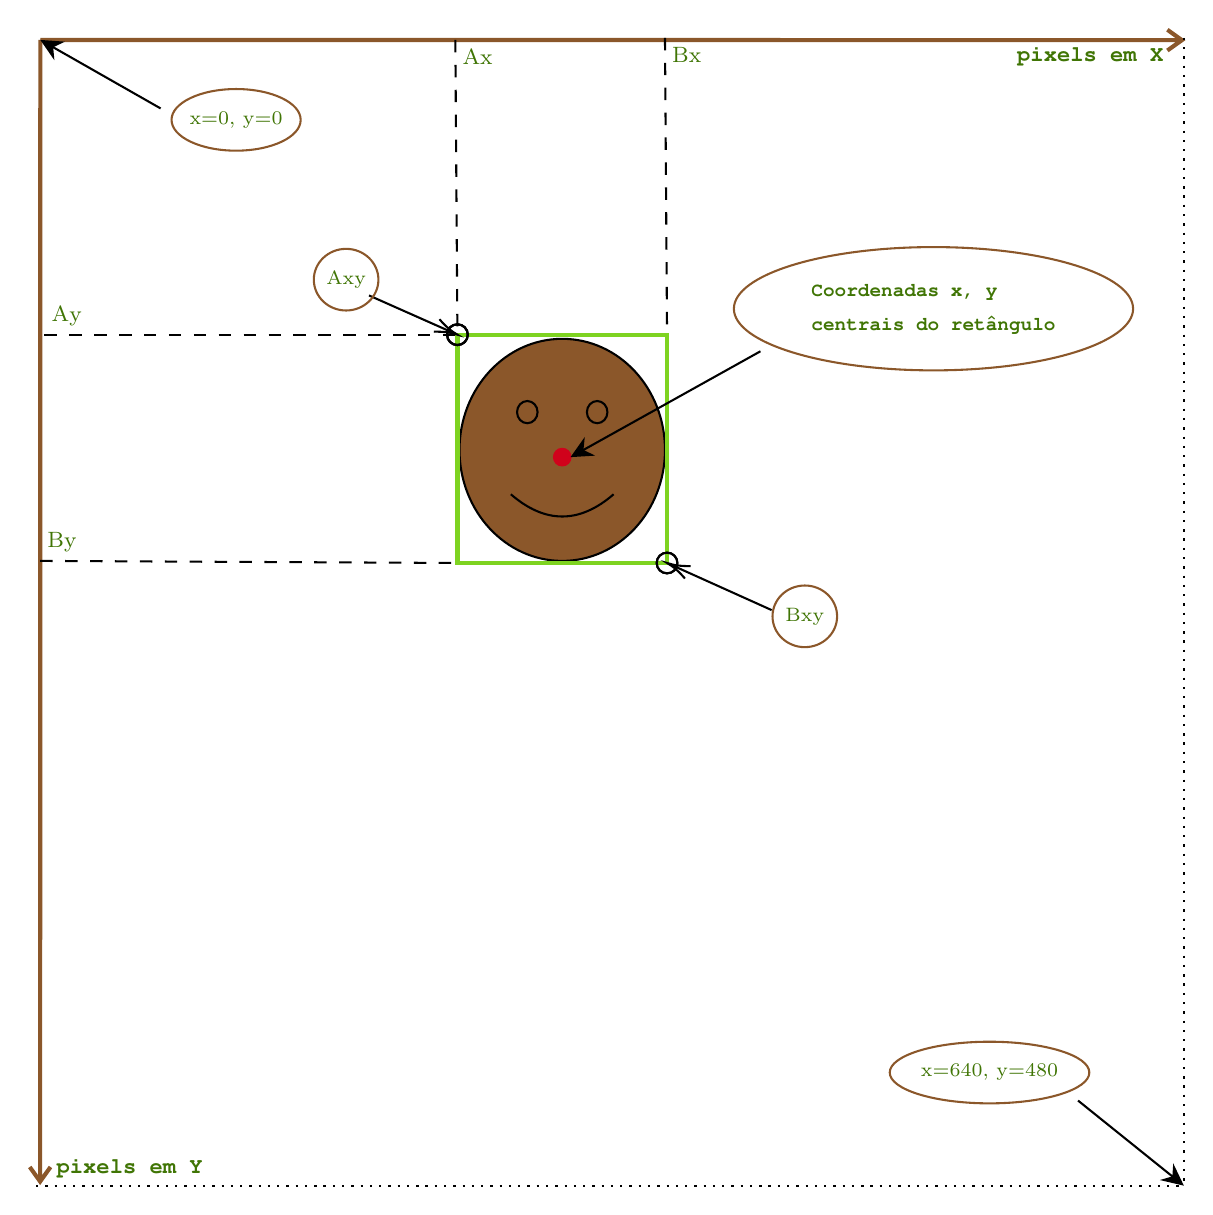
\begin{tikzpicture}[x=0.75pt,y=0.75pt,yscale=-1,xscale=1]
%uncomment if require: \path (0,802); %set diagram left start at 0, and has height of 802

%Shape: Axis 2D [id:dp4555798124742032] 
\draw [color={rgb, 255:red, 139; green, 87; blue, 42 }  ,draw opacity=1 ][line width=1.5]  (69.05,49.5) -- (68.95,599.5)(619.05,49.6) -- (69.05,49.5) -- cycle (73.95,592.5) -- (68.95,599.5) -- (63.95,592.5) (612.05,44.59) -- (619.05,49.6) -- (612.05,54.59)  ;
%Shape: Smiley Face [id:dp9391359153155296] 
\draw  [fill={rgb, 255:red, 139; green, 87; blue, 42 }  ,fill opacity=1 ] (271,247) .. controls (271,217.45) and (293.16,193.5) .. (320.5,193.5) .. controls (347.84,193.5) and (370,217.45) .. (370,247) .. controls (370,276.55) and (347.84,300.5) .. (320.5,300.5) .. controls (293.16,300.5) and (271,276.55) .. (271,247) -- cycle ; \draw  [fill={rgb, 255:red, 139; green, 87; blue, 42 }  ,fill opacity=1 ] (298.72,228.81) .. controls (298.72,225.86) and (300.94,223.46) .. (303.67,223.46) .. controls (306.4,223.46) and (308.62,225.86) .. (308.62,228.81) .. controls (308.62,231.76) and (306.4,234.16) .. (303.67,234.16) .. controls (300.94,234.16) and (298.72,231.76) .. (298.72,228.81) -- cycle ; \draw  [fill={rgb, 255:red, 139; green, 87; blue, 42 }  ,fill opacity=1 ] (332.38,228.81) .. controls (332.38,225.86) and (334.6,223.46) .. (337.33,223.46) .. controls (340.06,223.46) and (342.28,225.86) .. (342.28,228.81) .. controls (342.28,231.76) and (340.06,234.16) .. (337.33,234.16) .. controls (334.6,234.16) and (332.38,231.76) .. (332.38,228.81) -- cycle ; \draw   (295.75,268.4) .. controls (312.25,282.67) and (328.75,282.67) .. (345.25,268.4) ;
%Flowchart: Process [id:dp39379292608490624] 
\draw  [color={rgb, 255:red, 126; green, 211; blue, 33 }  ,draw opacity=1 ][line width=1.5]  (270,191.5) -- (371,191.5) -- (371,301.5) -- (270,301.5) -- cycle ;
%Straight Lines [id:da3834962043936656] 
\draw  [dash pattern={on 0.84pt off 2.51pt}]  (620,48.5) -- (620,601.5) ;
%Straight Lines [id:da28721230743083104] 
\draw  [dash pattern={on 0.84pt off 2.51pt}]  (67,601.5) -- (620,601.5) ;
%Straight Lines [id:da5550623511504473] 
\draw  [dash pattern={on 4.5pt off 4.5pt}]  (69,300.5) -- (270,301.5) ;
%Straight Lines [id:da3939101175382884] 
\draw  [dash pattern={on 4.5pt off 4.5pt}]  (71,191.5) -- (270,191.5) ;
%Straight Lines [id:da2141409001446355] 
\draw  [dash pattern={on 4.5pt off 4.5pt}]  (269,49.5) -- (270,191.5) ;
%Straight Lines [id:da6633828936036013] 
\draw  [dash pattern={on 4.5pt off 4.5pt}]  (370,48.5) -- (371,191.5) ;
%Shape: Circle [id:dp6494670108776119] 
\draw  [color={rgb, 255:red, 208; green, 2; blue, 27 }  ,draw opacity=1 ][fill={rgb, 255:red, 208; green, 2; blue, 27 }  ,fill opacity=1 ] (316.5,250.5) .. controls (316.5,248.29) and (318.29,246.5) .. (320.5,246.5) .. controls (322.71,246.5) and (324.5,248.29) .. (324.5,250.5) .. controls (324.5,252.71) and (322.71,254.5) .. (320.5,254.5) .. controls (318.29,254.5) and (316.5,252.71) .. (316.5,250.5) -- cycle ;
%Straight Lines [id:da15209721546831734] 
\draw    (416,199.5) -- (327.12,249.04) ;
\draw [shift={(324.5,250.5)}, rotate = 330.87] [fill={rgb, 255:red, 0; green, 0; blue, 0 }  ][line width=0.08]  [draw opacity=0] (10.72,-5.15) -- (0,0) -- (10.72,5.15) -- (7.12,0) -- cycle    ;
%Straight Lines [id:da4691908809525298] 
\draw    (127,82.5) -- (71.65,50.98) ;
\draw [shift={(69.05,49.5)}, rotate = 389.65999999999997] [fill={rgb, 255:red, 0; green, 0; blue, 0 }  ][line width=0.08]  [draw opacity=0] (10.72,-5.15) -- (0,0) -- (10.72,5.15) -- (7.12,0) -- cycle    ;
%Straight Lines [id:da8244683672036353] 
\draw    (569,560.5) -- (617.66,599.62) ;
\draw [shift={(620,601.5)}, rotate = 218.8] [fill={rgb, 255:red, 0; green, 0; blue, 0 }  ][line width=0.08]  [draw opacity=0] (10.72,-5.15) -- (0,0) -- (10.72,5.15) -- (7.12,0) -- cycle    ;
%Straight Lines [id:da7964680967109363] 
\draw [color={rgb, 255:red, 0; green, 0; blue, 0 }  ,draw opacity=0 ][fill={rgb, 255:red, 0; green, 0; blue, 0 }  ,fill opacity=0 ]   (371,301.5) -- (371,292.2) ;
%Straight Lines [id:da01751891515099846] 
\draw    (227.4,172.6) -- (268.17,190.69) ;
\draw [shift={(270,191.5)}, rotate = 203.93] [color={rgb, 255:red, 0; green, 0; blue, 0 }  ][line width=0.75]    (10.93,-3.29) .. controls (6.95,-1.4) and (3.31,-0.3) .. (0,0) .. controls (3.31,0.3) and (6.95,1.4) .. (10.93,3.29)   ;
%Straight Lines [id:da05405515080457568] 
\draw    (421.4,324.2) -- (372.82,302.32) ;
\draw [shift={(371,301.5)}, rotate = 384.25] [color={rgb, 255:red, 0; green, 0; blue, 0 }  ][line width=0.75]    (10.93,-3.29) .. controls (6.95,-1.4) and (3.31,-0.3) .. (0,0) .. controls (3.31,0.3) and (6.95,1.4) .. (10.93,3.29)   ;

% Text Node
\draw  [color={rgb, 255:red, 139; green, 87; blue, 42 }  ,draw opacity=1 ]  (526.37, 547) circle [x radius= 48.08, y radius= 14.85]   ;
\draw (526.37,547) node   [align=left] {{\scriptsize \textcolor[rgb]{0.25,0.46,0.02}{{\fontfamily{helvet}\selectfont x=640, y=480}}}};
% Text Node
\draw  [color={rgb, 255:red, 139; green, 87; blue, 42 }  ,draw opacity=1 ]  (437.37, 327.2) circle [x radius= 15.56, y radius= 14.85]   ;
\draw (437.37,327.2) node   [align=left] {{\scriptsize \textcolor[rgb]{0.25,0.46,0.02}{{\fontfamily{helvet}\selectfont Bxy}}}};
% Text Node
\draw  [color={rgb, 255:red, 139; green, 87; blue, 42 }  ,draw opacity=1 ]  (216.37, 165) circle [x radius= 15.56, y radius= 14.85]   ;
\draw (216.37,165) node   [align=left] {{\scriptsize \textcolor[rgb]{0.25,0.46,0.02}{{\fontfamily{helvet}\selectfont Axy}}}};
% Text Node
\draw  [color={rgb, 255:red, 139; green, 87; blue, 42 }  ,draw opacity=1 ]  (163.37, 88) circle [x radius= 31.11, y radius= 14.85]   ;
\draw (163.37,88) node   [align=left] {{\scriptsize \textcolor[rgb]{0.25,0.46,0.02}{{\fontfamily{helvet}\selectfont x=0, y=0}}}};
% Text Node
\draw  [color={rgb, 255:red, 139; green, 87; blue, 42 }  ,draw opacity=1 ]  (499.37, 179) circle [x radius= 96.17, y radius= 29.7]   ;
\draw (499.37,179) node   [align=left] {{\scriptsize \textcolor[rgb]{0.25,0.46,0.02}{\textbf{{\fontfamily{pcr}\selectfont Coordenadas x, y}}}}\\{\scriptsize \textcolor[rgb]{0.25,0.46,0.02}{\textbf{{\fontfamily{pcr}\selectfont centrais do retângulo}}}}};
% Text Node
\draw (69,598.5) node [anchor=south west] [inner sep=0.75pt]   [align=left] {{\footnotesize \textbf{\textcolor[rgb]{0.25,0.46,0.02}{{\fontfamily{pcr}\selectfont  \ pixels em Y}}}}};
% Text Node
\draw (618,51.5) node [anchor=north east] [inner sep=0.75pt]   [align=left] {{\footnotesize \textbf{\textcolor[rgb]{0.25,0.46,0.02}{{\fontfamily{pcr}\selectfont pixels em X }}}}};
% Text Node
\draw (271,52.5) node [anchor=north west][inner sep=0.75pt]   [align=left] {{\fontfamily{helvet}\selectfont {\footnotesize \textcolor[rgb]{0.25,0.46,0.02}{Ax}}}};
% Text Node
\draw (73,188.5) node [anchor=south west] [inner sep=0.75pt]   [align=left] {{\fontfamily{helvet}\selectfont {\footnotesize \textcolor[rgb]{0.25,0.46,0.02}{Ay}}}};
% Text Node
\draw (71,297.5) node [anchor=south west] [inner sep=0.75pt]   [align=left] {{\fontfamily{helvet}\selectfont {\footnotesize \textcolor[rgb]{0.25,0.46,0.02}{By}}}};
% Text Node
\draw (372,51.5) node [anchor=north west][inner sep=0.75pt]   [align=left] {{\fontfamily{helvet}\selectfont {\footnotesize \textcolor[rgb]{0.25,0.46,0.02}{Bx}}}};

\draw   (270, 191.5) circle [x radius= 5, y radius= 5]   ;
\draw   (270, 191.5) circle [x radius= 5, y radius= 5]   ;
\draw   (270, 191.5) circle [x radius= 5, y radius= 5]   ;
\draw   (371, 301.5) circle [x radius= 5, y radius= 5]   ;
\draw   (371, 301.5) circle [x radius= 5, y radius= 5]   ;
\end{tikzpicture}
